\documentclass[a4paper,14pt]{report}
\usepackage[utf8]{inputenc}
\usepackage[T1]{fontenc}
\usepackage{titlesec}
\usepackage{amsmath}
\usepackage{float}
\usepackage{amssymb}
\usepackage{graphicx}

\usepackage{algorithm}
\usepackage{algorithmic}


\graphicspath{ {./wykresy/} }

\renewcommand{\contentsname}{Spis treści}

\titleformat{\chapter}[display]
  {\normalfont\bfseries}{}{0pt}{\Huge}

\usepackage{pgfplots}
 
\pgfplotsset{compat = newest}

\title{Obliczenia naukowe Lista 5}
\author{Radosław Wojtczak}
\date{Numer indeksu: 254607}
\begin{document}
\maketitle
\tableofcontents
\chapter{Omówienie problematyki}
  Problematyka zadania opierała się na efektywnym (pod względem złożoności obliczeniowej jak i pamięciowej) rozwiązaniu układu równań liniowych postaci:
  \begin{equation}
    \textbf{Ax}=\textbf{b}
  \end{equation} 
  dla szczególnej postaci macierzy \textbf{A} ($\mathbf{A} \in \mathbb{R}^{n \times n})$: \\
  \begin{figure}[H]
  \centering
  $ \begin{bmatrix}
    \mathbf{A_1} & \mathbf{C_1} & \mathbf{0} & \mathbf{0} & \mathbf{0} & \mathbf{...} & \mathbf{0} \\
    \mathbf{B_2} & \mathbf{A_2} & \mathbf{C_2} & \mathbf{0} & \mathbf{0} & \mathbf{...} & \mathbf{0} \\
    \mathbf{0} & \mathbf{B_3} & \mathbf{A_3} & \mathbf{C_3} & \mathbf{0} & \mathbf{...} & \mathbf{0} \\
    \mathbf{...} & \mathbf{...} & \mathbf{...} & \mathbf{...} & \mathbf{...} & \mathbf{...} & \mathbf{...} \\
    \mathbf{0} & \mathbf{...} & \mathbf{0} & \mathbf{B_{v-2}} & \mathbf{A_{v-2}} & \mathbf{C_{v-2}} & \mathbf{0} \\
    \mathbf{0} & \mathbf{...} & \mathbf{0} & \mathbf{0} & \mathbf{B_{v-1}} & \mathbf{A_{v-1}} & \mathbf{C_{v-1}} \\
    \mathbf{}0 & \mathbf{...} & \mathbf{0} & \mathbf{0} & \mathbf{0} & \mathbf{B_{v}} & \mathbf{A_{v}} 
  \end{bmatrix}  $  
  \end{figure}
  oraz wektora prawych stron \textbf{b} ($\mathbf{b} \in \mathbb{R}^{n}$). Macierze $\mathbf{A_{k},B_{k},C_{k}}$ są następujących postaci:
  \begin{enumerate}
    \item Macierz $\mathbf{A_{k}}$, $k =1,...,v$,gdzie $v=n/l$, przy założeniu, że n jest podzielne przez l oraz $l \geq 2$, jest macierzą gęstą (oznacza to, że ów macierz ma wszystkie elementy niezerowe)
    \item Macierz $\mathbf{B_{k}}$, $k=2,...,v$ (v jak powyżej) jest macierzą zawierającą jedyne niezerowe elementy umieszczone w dwóch ostatnich kolumnach
    \item Macierz $\mathbf{C_{k}}$, $k=1,...,v-1$ (v jak powyzej) jest macierzą diagonalną

  \end{enumerate}
  Dodatkowo macierze \textbf{0} są macierzami kwadratowymi zerowego stopnia l.
  W pierwszej części zadania, do rozwiązania układu liniowego z tak specyficzną specyfikacją macierzy \textbf{A}, należało odpowiednio zmodyfikować metodę eliminacji Gaussa dla dwóch wariantów:
  \begin{itemize}
    \item bez wyboru elementu głównego
    \item z częsciowym wyborem elementu głównego
  \end{itemize}
  W drugiej zaś należało wyznaczyć rozkład \textbf{LU} macierzy \textbf{A} przy pomocy wcześniej zmodyfikowanej metody eliminacji Gaussa (również jak w przypadku Gaussa dla dwóch wariantów- z, jak i z częściowym wyboremelementu głównego) oraz napisać funkcję rozwiązującą zadany układ równań dla wcześniej wyznaczonego rozkładu \textbf{LU} przez powyżej wspomnianą funkcję. \\
  Dalsza część tego dokumentu będzie składała się z omówienia poszczególnych części wchodzących w skład zadania oraz przedstawienia, jak i zinterpetowania otrzymanych wyników. \\
  Wszystkie funkcje zostały zaimplementowane w module o nazwie \textbf{blocksys.jl}, zgodnie z poleceniem zadania. Rozwiązanie wykorzystuje gotową strukturę danych o nazwie \textit{SparseArray}, która w efektywny sposób pozwala nam na zapamiętanie niezerowych elementów macierzy. \\
  Pliki
  \begin{itemize}
    \item gaussTest.jl
    \item gaussPivotTest.jl
    \item LuTest.jl
    \item LuPivotTest.hl
  \end{itemize}
  implementują testy odpowiednio dla: metody eliminacji gausa bez wyboru elementu głównego, z częściowym wyborem elementu głównego, rozkładu \textbf{LU} bez elementu głównego, z częściowym wyborem elementu głównego. 
  Testy wykorzystują dostarczony z poleceniem zadania moduł \textbf{matrixgen.jl)} zawierający funkcję \textbf{blockmat()} odpowiedzialną za generowanie odpowiednich macierzy. Testy wykonywane są dla $n \in \{1000,1010,1020,...,50000\}$ oraz stałego $l=4$. Sprawdzany jest czas, jak i wykorzystana pamięć, przez każdą z funkcji w trakcie rozwiązywania układu równań.
\chapter{Eliminacja Gaussa}
  \section{Wprowadzenie}
  Metoda eliminacja Gaussa jest algorytmem stosowanym do rozwiązywania układów równań liniowych jak i wyznaczania rozkładu LU, wykorzystując operacje elementarne. Operacje elementarne wykonywane na macierzach to:
  \begin{itemize}
    \item Dodawanie do jednego wiersza macierzy innego wiersza pomnożonego przez liczbę
    \item zamienienie dwóch wierszy miejscami
    \item pomnożenie wierszy przez liczbę różną od zera
  \end{itemize}
  W ów zadaniu podstawowy algorytm eliminacji Gaussa należało zmodyfikować tak, aby wykorzystywał specyficzną strukturę macierzy w celu szybszej realizacji postawionego problemu. Analizę zaczniemy od wizualizacji macierzy dla następujących danych wejściowych: $n=16$, $l=4$, z czego automatycznie otrzymujemy $v=4$.
  \begin{figure}[H]
      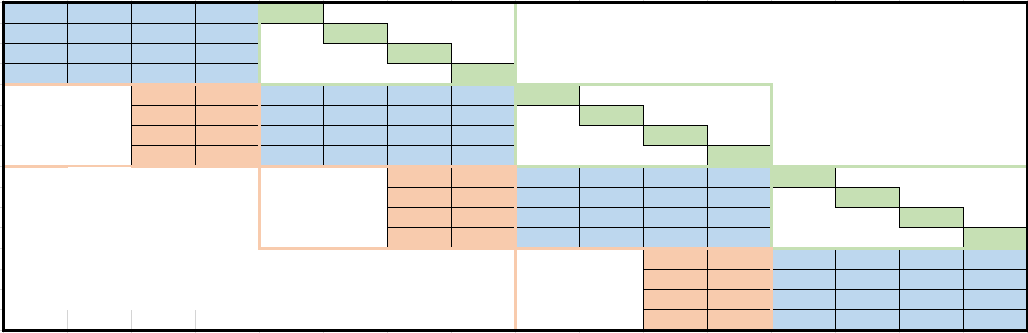
\includegraphics[scale=0.5]{macierz}
      \centering
      \caption{Struktura macierzy dla $n=16$ oraz $l=4$}
    \end{figure}
  Białym wypełnieniem oznaczone są komórki, w których znajdują się wartości zerowe. Obramowaniem jasnoniebieskim oznaczone są macierze $\mathbf{A_{k}}$
, jasnopomarańczowym- $\mathbf{B_{k}}$, a $\mathbf{C_{k}}$- jasnozielonym. Dodatkowo komórki, które w tych macierzach są niezerowane zostały wypełnione kolorem odpowiadającym kolorowi obramowania.
  Pierwszym spostrzeżeniem jest fakt, iż liczba elementów niezerowych zależy od liczby l. Dodatkowo zauważamy, że
  \begin{itemize}
    \item Każda z macierzy $\mathbf{A_{k}}$ składa się z $l^{2}$ elementów niezerowych 
    \item Każda z macierzy $\mathbf{B_{k}}$ składa się z $2*l$ elementów niezerowych
    \item Każda z macierzy $\mathbf{C_{k}}$ składa się z $l$ elementów niezerowych
  \end{itemize}
  Wiedząc, że v oznacza liczbę takich macierzy możemy obliczyć sumę niezerowych komórek dla danej macierzy \textbf{A}:
  $v*l^{2}+(v-1)*2*l+(v-1)*l=n/l*l^{2}+(n/l-1)*2*l+(n/l-1)*l=n*l+2*n-2*l+n-l=n*l+3*n-3*l=n*l+3(n-l)$ co pomoże nam w dokładnym alokowaniu wektorów w dalszym działaniu programu.
  \section{Analiza algorytmu}
  Pseudokod algorytmu zaimplementowanego w module \textbf{blocksys.jl} w funkcji \textbf{gauss()}:

  \begin{algorithm}[H]
    \caption{Metoda eliminacji Gaussa}
    \textbf{INPUT:}
    \begin{itemize}
      \item matrix- struktura typu \textit{SparseArray}
      \item b- wektor prawych stron 
      \item n- rozmiar macierzy
      \item l- rozmiar bloku wewnętrznego
    \end{itemize}
    \textbf{OUTPUT:}
    \begin{itemize}
      \item result- wektor o rozmiarze n zawierający pierwiastki równania
    \end{itemize}
    \begin{algorithmic} 
      \FOR{$k \leftarrow 1$ \textbf{to} $n-1$}
        \FOR{$i \leftarrow k+1$ \textbf{to} $min(n,k+l+1)$}
          \IF{eps(Float64)>abs(matrix[k,k])}
            \STATE \textbf{print}:Zero w mianowniku
            \STATE \textbf{break}
          \ENDIF
          \STATE $I \leftarrow matrix[i,k]/matrix[k,k]$
          \STATE $matrix[i,k] \leftarrow 0$
          \FOR{$j \leftarrow k+1$ \textbf{to} $min(n,k+l)$}
            \STATE $matrix[i,j] \leftarrow matrix[i,j]-I*matrix[k,j]$
          \ENDFOR
          \STATE $b[i] \leftarrow b[i]-I*b[k]$
        \ENDFOR
        \STATE $result \leftarrow Array[n]=\{0\}$
        \FOR{$a \leftarrow n$ \textbf{downto} $1$}
          \STATE $sum \leftarrow 0$
          \FOR{$z \leftarrow a+1$ \textbf{to} $min(n,a+l)$}
            \STATE $sum \leftarrow sum+matrix[a,z]*result[z]$
          \ENDFOR
          \STATE $result[a] \leftarrow (b[a]-sum)/matrix[a,a]$
        \ENDFOR
      \ENDFOR
      \RETURN result
      \end{algorithmic}
  \end{algorithm}
  Algorytm rozpoczynamy pętlą przechodzącą po wszystkich kolumnach macierzy. Kolejna pętla- wewnętrzna, odpowiada za iterowanie po wierszach. Tutaj korzystamy z własności macierzy i zauważamy, iż liczba elementów do sprawdzenia w danym wierszu jest nie większa niż l+1. Następnie pod zmienną \textit{I} podstawiamy wynik dzielenia aktualnie rozpatrywanego wiersza w danej kolumnie z wartością diagonalną po czym zerujemy aktualnie rozpatrywaną komórkę. Notacja matrix[a,b] jest równoważna elementowi w rzędzie \textbf{a} (numerowanym od 1) i kolumnie \textbf{b}. Po wyelimowaniu zmiennej z równania przechodzimy do odejmowania I od pozostałych wyrazów w danym wierszu. \\
  Po zakończeniu działania pierwszej pętli \textbf{FOR} otrzymujemy macierz górnotrójkątną. Następnie deklarujemy tablicę o nazwie \textbf{result}, w której będziemy przechowywać pierwiastki równania. W drugiej pętli \textbf{FOR} przechodzimy wstecz, wyliczając pierwiastki od ostatniego do pierwszego. Taką metodę postępowania nazywamy \textbf{podstawianiem wstecz}.
  Po wykonaniu drugiej pętli \textbf{FOR} w tablicy \textbf{result} znajdują się wszystkie pierwistki równania, której zwracamy użytkownikowi. W tym momencie funkcja kończy swoje działanie pomyślnie.

  \textbf{Złożoność:}
  W algorytmie Gaussa przechodzimy po przekątnej macierzy, zerując elementy, które się pod nią znajdują. Nie posiadając żadnych dodatkowych informacji na temat obsługiwanych macierzy zauważamy, że każda z wewnętrznych pętli \textbf{for} musiałaby zostać wykonana aż do końca macierzy, czyli do $n$. To dałoby nam złożonośc na poziomie $\mathbf{O(n^{3})}$. W tym miejscu korzystamy z specyfikacji zadania. Szybko zauważamy, że w takim przypadku maksymalna liczba elementów do rozpatrzenia w każdym wierszu, jak i w każdej kolumnie jest równa $l+1$. Oczywistym jest, ów liczba nie jest stała- przykładem będzie chociażby pierwsza kolumna dla $l=4$. W tej sytuacji macierz \textbf{B} ma niezerowe elementy jedynie w kolumnie 3 i 4 macierzy \textbf{A}, więc wystarczyłoby rozpatrzeć jedynie l elementów, jednakże implementacja korzysta z uproszczenia i wszystkie pętle rozpatrują $l+1$ elementów (z wyjątkiem sytuacji, w których n jest liczbą mniejszą niż $l+1$- wtedy wychodzilibyśmy poza ramy tablicy, co kończyłoby się błędem kompilacji). Oznacza to, że przyjmując $l$ jako liczbę stałą schodzimy ze złożoności $\mathbf{O(n^{3})}$ na $\mathbf{O(n*(l^{2}+l))}$, co uznajemy jako $\mathbf{O(n)}$. \\
  Ze względu na to, że macierz składa się z $n*l+3(n-l)$ elementów niezerowych (a tylko takie zapamiętujemy) łatwo zauważamy, iż złożonośc pamięciowa wynosi \textbf{O(n)}. 





\chapter{Eliminacja Gaussa z częściowym wyborem}
  \section{Wprowadzenie}
  W tym przypadku dokonujemy drobnej modyfikacji standardowego algorytmu rozwiązywania układu równań metodą eliminacji Gaussa. Wprowadzamy nowe pojęcie częściowego wyboru, który polega na znalezieniu elementu, które jest największy co do wartości bezwzględnej w danym wierszu. Następnie takowy znaleziony element determinuje nam wiersz, który zamieniamy z wierszem aktualnie rozpatrywanym. Przestawienie dotyczy się również macierzy prawych stron. \\
  W ten sposób zmniejszamy błędy wynikające z niedokładnej reprezentacji liczb zmiennoprzecinkowych w komputerach. Dzięki wyborowi elementu o największej co do wartości bezwzględnej wartości zmniejszamy szansę na wykonywanie działań na bardzo małych liczbach (co, jak pokazywaliśmy wielokrotnie w trakcie wykonywania zadań na ów kursie, może drastycznie wpływać na otrzymane wyniki)

  \section{Analiza algorytmu}
  Pseudokod algorytmu zaimplementowanego w module \textbf{blocksys.jl} w funkcji \textbf{gaussPivot()}:
  \begin{algorithm}[H]
    \caption{Metoda eliminacji Gaussa z wykorzystaniem częściowego wyboru elementu głównego}
    \textbf{INPUT:}
    \begin{itemize}
      \item matrix- struktura typu \textit{SparseArray}
      \item b- wektor prawych stron 
      \item n- rozmiar macierzy
      \item l- rozmiar bloku wewnętrznego
    \end{itemize}
    \textbf{OUTPUT:}
    \begin{itemize}
      \item result- wektor o rozmiarze n zawierający pierwiastki równania
    \end{itemize}
    \begin{algorithmic} 
      \STATE $pivot \leftarrow \{1,...,n\}$
      \FOR{$k \leftarrow 1$ \textbf{to} $n-1$}
        \STATE $row \leftarrow k$
        \STATE $value=abs(matrix[pivot[k],k])$
        \FOR{$i \leftarrow k+1$ \textbf{to} $min(n,k+l+1)$}
          \IF{$abs(matrix[pivot[i],k])>value$}
            \STATE $value \leftarrow matrix[pivot[i],k]$
            \STATE $row \leftarrow i$
          \ENDIF
        \ENDFOR

        \STATE $pivot[row],pivot[k] \leftarrow pivot[k],pivot[row]$



        \FOR{$i \leftarrow k+1$ \textbf{to} $min(n,k+l+l+1)$}
          \IF{eps(Float64)>abs(matrix[pivot[k],k])}
            \STATE \textbf{print}:Zero w mianowniku
            \STATE \textbf{break}
          \ENDIF
          \STATE $I \leftarrow matrix[pivot[i],k]/matrix[pivot[k],k]$
          \STATE $matrix[pivot[i],k] \leftarrow 0$
          \FOR{$j \leftarrow k+1$ \textbf{to} $min(n,k+l+l)$}
            \STATE $matrix[pivot[i],j] \leftarrow matrix[pivot[i],j]-I*matrix[pivot[k],j]$
          \ENDFOR
          \STATE $b[pivot[i]] \leftarrow b[pivot[i]]-I*b[pivot[k]]$
        \ENDFOR
        \STATE $result \leftarrow Array[n]=\{0\}$
        \FOR{$a \leftarrow n$ \textbf{downto} $1$}
          \STATE $sum \leftarrow 0$
          \FOR{$z \leftarrow a+1$ \textbf{to} $min(n,a+l+l)$}
            \STATE $sum \leftarrow sum+matrix[pivot[a],z]*result[z]$
          \ENDFOR
          \STATE $result[a] \leftarrow (b[pivot[a]]-sum)/matrix[pivot[a],a]$
        \ENDFOR
      \ENDFOR
      \RETURN result
      \end{algorithmic}
  \end{algorithm}
  Na pierwszy rzut oka spostrzegamy duże podpobieństwo względem poprzedniego algorytmu. Różnice jednak występują w dodaniu specjalnej tablicy, której początkowymi elementami są liczby naturalne od 1 do n o nazwie \textit{pivot}, która ma za zadanie przechowywać rotację w indeksach po ustaleniu częściowego elementu głównego. Konsekwencją tego jest dodanie dodatkowej pętli \textbf{FOR} w linii numer 5, oraz dwóch zmiennych lokalnych: \textit{row}, która przechowuje wiersz, w którym znajduje się maksymalna co do wartości bezwzględnej wartość, oraz \textit{value}, która ów wartość przechowuje. Ustalenie elementu maksymalnego zachodzi w trywialny sposób- liniowo porównujemy wszystkie elementy zapamiętując największy. W reszcie algorytmu w kolumnie wierszy wszystkie napisy z \textbf{x} zostały zamienione na \textbf{pivot[x]}, gdyż to właśnie tablica \textit{pivot} przechowuje indeksy po zmianie.
  \textbf{Złożoność:}
  W algorytmie Gaussa z częściowym wyborem elementu głównego dochodzi nam jeden \textbf{FOR} na drugim poziomie zagnieżdżenia, która wykonuje się zawsze $l+1$ razy. Dodatkowo we wszystkich późniejszych pętlach \textbf{FOR} na poziomie drugim liczba sprawdzanych indeksów wzrosła o l (z $l+1$ do $l+l+1$). Wynika to z faktu, iż mogło dojść do zamiany wiersza k-tego z wierszem k+l-tym. W tej sytuacji dochodzi do zamian w całych wierszach, co ma znaczenie ze względu na strukturę macierzy $\mathbf{C_{k}}$, która jest macierzą diagonalną. Weźmy pod uwagę sytuację, gdy k=1, a maksymalna wartość znajduje się k=l. Wtedy należy zamienić ze sobą wiersze 1 i l, co prowadzi również do zamiany elementów znajdujących się w macierzy $\mathbf{C_{k}}$- w rozpatrywanym wierszu ostatni element będzie znajdował się na pozycji k+l-tej. \\
  Z teoretycznego punktu widzenia ów zmiana nie wpływa na złożoność obliczeniową, która dalej wynosi \textbf{O(n)}, przy założeniu, że l jest liczbą stałą. Zwiększy się jedynie współczynnik stojący przy wyrazie n, jednakże nie wpływa to na asymptotykę ów funkcji.
  Ze względu na to, iż macierz składa się z $n*l+3(n-l)$ elementów niezerowych (a tylko takie zapamiętujemy) łatwo zauważamy, iż złożonośc pamięciowa wynosi \textbf{O(n)}. 



\chapter{Rozkład LU}
  \section{Wprowadzenie}
  Rozkład \textbf{LU} (ang. lower-upper) polega na rozłożeniu macierzy kwadratowej na iloczyn dwóch macierzy trójkątnych- macierzy dolnotrójątknej 
  \textbf{L} (której elementy diagonalne są równe 1) oraz macierzy górnotrójkątnej \textbf{U}. Z wykładu wiemy, iż Eliminację Gaussa możemy traktować jako algorytm rozkładu trójkątnego.\\
  $\mathbf{A}^{(n)}=\mathbf{L}^{(n-1)}...\mathbf{L}^{(2)}*\mathbf{L}^{(1)}*\mathbf{A}^{(1)}$
  gdzie zapis $\mathbf{A}^{(n)}$ oznacza stan macierzy $\mathbf{A}$ po $n-1$ krokach. \\
  Następnie oznaczamy przez $\mathbf{U}$ - $\mathbf{A}^{(n)}$. Wychodząc z $\mathbf{A}=\mathbf{A}^{(1)}$ otrzymujemy:
  $\mathbf{U}=\mathbf{L}^{(n-1)}...\mathbf{L}^{(2)} \mathbf{L}^{(1)}\mathbf{A}^{(1)}$, $\mathbf{A}=\mathbf{L}^{(1)^{-1}}\mathbf{L}^{(2)^{-1}}...\mathbf{L}^{(n-1)^{-1}}\mathbf{U}$ \\
  gdzie $\mathbf{L}=\mathbf{L}^{(1)^{-1}}\mathbf{L}^{(2)^{-1}}...\mathbf{L}^{(n-1)^{-1}}.$ \\
  Z tego od razu wnioskujemy, iż eliminacja Gaussa jest równoważna rozkładowi macierzy na postać \textbf{LU}
  \section{Analiza algorytmu}
  Ze względu na polecenie zadania funkcja \textbf{LU()} wyznacza rozkład \textbf{LU} macierzy \textbf{A} metodą eliminacji Gaussa, natomiast funkcja \textbf{LUSolver()} rozwiązuje układ równań $\mathbf{Ax=b}$ dla wcześniej wyznaczonego rozkładu \textbf{LU}\\
  \section{LU()}
  Pseudokod algorytmu zaimplementowanego w module \textbf{blocksys.jl} w funkcji \textbf{LU()}:
  \begin{algorithm}[H]
    \caption{rozkład LU}
    \textbf{INPUT:}
    \begin{itemize}
      \item matrix- struktura typu \textit{SparseArray}
      \item n- rozmiar macierzy
      \item l- rozmiar bloku wewnętrznego
    \end{itemize}
    \textbf{WYNIK:}
    \begin{itemize}
      \item Macierz w postaci \textbf{LU}
    \end{itemize}
    \begin{algorithmic} 
      \FOR{$k \leftarrow 1$ \textbf{to} $n-1$}
        \FOR{$i \leftarrow k+1$ \textbf{to} $min(n,k+l+1)$}
          \IF{eps(Float64)>abs(matrix[k,k])}
            \STATE \textbf{print}:Zero w mianowniku
            \STATE \textbf{break}
          \ENDIF
          \STATE $I \leftarrow matrix[i,k]/matrix[k,k]$
          \STATE $matrix[i,k] \leftarrow I$
          \FOR{$j \leftarrow k+1$ \textbf{to} $min(n,k+l)$}
            \STATE $matrix[i,j] \leftarrow matrix[i,j]-I*matrix[k,j]$
          \ENDFOR
          \STATE $b[i] \leftarrow b[i]-I*b[k]$
        \ENDFOR
      \ENDFOR
      \end{algorithmic}
  \end{algorithm}
  Zauważamy, iż jedyną różnicą między ów algorytmem, a algorytmem eliminacji Gaussa jest podstawienie za element $matrix[i,k]$ zmiennej \textbf{I}. Wynika to z faktu, iż macierz \textbf{U} na przekątnej posiada obliczone wartości, które przy łączeniu z macierzą \textbf{I} tworzą spójną całość. Należy zauważyć, iż wszystko trzymane jest w jednej macierzy, podział na dwie jest zbędny, co zostało pokazane we wcześniejszej sekcji, co prowadzi do efektywniejszego zapamiętywania rozkładu jeśli chodzi o wykorzystaną pamięć.
  \textbf{Złożoność:}
    Występujące pętle są tożsame z pętlami występującymi występującymi w funkcji \textbf{gauss()}, stąd wnioskujemy, iż złożoność pamięciowa jak i czasowa jest na poziomie \textbf{O(n)}.


  \section{LUSolver()}
  Pseudokod algorytmu zaimplementowanego w module \textbf{blocksys.jl} w funkcji \textbf{LUSolver()}:
  \begin{algorithm}[H]
    \caption{Metoda eliminacji Gaussa}
    \textbf{INPUT:}
    \begin{itemize}
      \item matrix- struktura typu \textit{SparseArray}
      \item b- wektor prawych stron 
      \item n- rozmiar macierzy
      \item l- rozmiar bloku wewnętrznego
    \end{itemize}
    \textbf{OUTPUT:}
    \begin{itemize}
      \item result- wektor o rozmiarze n zawierający pierwiastki równania
    \end{itemize}
    \begin{algorithmic} 
      \FOR{$k \leftarrow 1$ \textbf{to} $n-1$}
        \FOR{$i \leftarrow k+1$ \textbf{to} $min(n,k+l+1)$}
          \STATE $b[i] \leftarrow b[i]-matrix[i,k]*b[k]$
        \ENDFOR
        \STATE $result \leftarrow Array[n]=\{0\}$
        \FOR{$a \leftarrow n$ \textbf{downto} $1$}
          \STATE $sum \leftarrow 0$
          \FOR{$z \leftarrow a+1$ \textbf{to} $min(n,a+l)$}
            \STATE $sum \leftarrow sum+matrix[a,z]*result[z]$
          \ENDFOR
          \STATE $result[a] \leftarrow (b[a]-sum)/matrix[a,a]$
        \ENDFOR
      \ENDFOR
      \RETURN result
      \end{algorithmic}
  \end{algorithm}
  Ów algorytm jest tożsamy z drugą pętlą \textbf{FOR} na drugim poziomie zagnieżdżenia w algorytmie eliminacji gaussa. Również złożonośc pamięciowa jak i obliczeniowa ów algorytmu wynosi \textbf{O(n)}




\chapter{Rozkład LU z częściowym wyborem elementu głównego}
  \section{Wprowadzenie}
  Z podobnych powódek jak w metodzie eliminacji Gaussa, przy wykonywaniu rozkładu \textbf{LU} można zastosować wyznaczenie częściowego elementu głównego, w celu redukcji błędów związanych z zaokrągleniami oraz wykonywania obliczeń na liczbach bliskich zeru. Podobnie jak w przypadku Rozkładu LU bez częściowego wyboru postały dwie funkcje, \textbf{LUPivot()} wyznacza rozkład \textbf{LU} macierzy \textbf{A} metodą eliminacji Gaussa przy użyciu częściowego wyboru elementu głównego oraz funkcja \textbf{LUPivotSolver()} rozwiązująca układ równań $\mathbf{Ax=b}$ dla wcześniej wyznaczonego rozkładu \textbf{LU} z częściowym wyborem elementu głównego\\


  \section{LUPivot()}
  Pseudokod algorytmu zaimplementowanego w module \textbf{blocksys.jl} w funkcji \textbf{LUPivot()}:
    \begin{algorithm}[H]
    \caption{rozkład LU}
    \textbf{INPUT:}
    \begin{itemize}
      \item matrix- struktura typu \textit{SparseArray}
      \item n- rozmiar macierzy
      \item l- rozmiar bloku wewnętrznego
    \end{itemize}
    \textbf{OUTPUT:}
    \begin{itemize}
      \item pivot- Macierz indeksów
    \end{itemize}
    \begin{algorithmic} 
      \STATE $pivot \leftarrow \{1,...,n\}$
      \FOR{$k \leftarrow 1$ \textbf{to} $n-1$}
        \STATE $row \leftarrow k$
        \STATE $value=abs(matrix[pivot[k],k])$
        \FOR{$i \leftarrow k+1$ \textbf{to} $min(n,k+l+1)$}
          \IF{$abs(matrix[pivot[i],k])>value$}
            \STATE $value \leftarrow matrix[pivot[i],k]$
            \STATE $row \leftarrow i$
          \ENDIF
        \ENDFOR

        \STATE $pivot[row],pivot[k] \leftarrow pivot[k],pivot[row]$



        \FOR{$i \leftarrow k+1$ \textbf{to} $min(n,k+l+l+1)$}
          \IF{eps(Float64)>abs(matrix[pivot[k],k])}
            \STATE \textbf{print}:Zero w mianowniku
            \STATE \textbf{break}
          \ENDIF
          \STATE $I \leftarrow matrix[pivot[i],k]/matrix[pivot[k],k]$
          \STATE $matrix[pivot[i],k] \leftarrow I$
          \FOR{$j \leftarrow k+1$ \textbf{to} $min(n,k+l+l)$}
            \STATE $matrix[pivot[i],j] \leftarrow matrix[pivot[i],j]-I*matrix[pivot[k],j]$
          \ENDFOR
          \STATE $b[pivot[i]] \leftarrow b[pivot[i]]-I*b[pivot[k]]$
        \ENDFOR
        \STATE $result \leftarrow Array[n]=\{0\}$
        \FOR{$a \leftarrow n$ \textbf{downto} $1$}
          \STATE $sum \leftarrow 0$
          \FOR{$z \leftarrow a+1$ \textbf{to} $min(n,a+l+l)$}
            \STATE $sum \leftarrow sum+matrix[pivot[a],z]*result[z]$
          \ENDFOR
          \STATE $result[a] \leftarrow (b[pivot[a]]-sum)/matrix[pivot[a],a]$
        \ENDFOR
      \ENDFOR
      \RETURN result
      \end{algorithmic}
  \end{algorithm}


  \section{LUSolver()}
  Pseudokod algorytmu zaimplementowanego w module \textbf{blocksys.jl} w funkcji \textbf{LUSolver()}:
  \begin{algorithm}[H]
    \caption{Metoda eliminacji Gaussa}
    \textbf{INPUT:}
    \begin{itemize}
      \item matrix- struktura typu \textit{SparseArray}
      \item b- wektor prawych stron 
      \item n- rozmiar macierzy
      \item l- rozmiar bloku wewnętrznego
    \end{itemize}
    \textbf{OUTPUT:}
    \begin{itemize}
      \item result- wektor o rozmiarze n zawierający pierwiastki równania
    \end{itemize}
    \begin{algorithmic} 
      \FOR{$k \leftarrow 1$ \textbf{to} $n-1$}
        \FOR{$i \leftarrow k+1$ \textbf{to} $min(n,k+l+1)$}
          \STATE $b[i] \leftarrow b[i]-matrix[i,k]*b[k]$
        \ENDFOR
        \STATE $result \leftarrow Array[n]=\{0\}$
        \FOR{$a \leftarrow n$ \textbf{downto} $1$}
          \STATE $sum \leftarrow 0$
          \FOR{$z \leftarrow a+1$ \textbf{to} $min(n,a+l)$}
            \STATE $sum \leftarrow sum+matrix[a,z]*result[z]$
          \ENDFOR
          \STATE $result[a] \leftarrow (b[a]-sum)/matrix[a,a]$
        \ENDFOR
      \ENDFOR
      \RETURN result
      \end{algorithmic}
  \end{algorithm}

  Analogicznie do sytuacji z metodą eliminacji Gaussa- \textbf{O(n)} jest złożonością zarówno pamięciową jak i czasową.

\chapter{Wyniki i interpretacje}
  Poniższe wykresy przedstawiają otrzymane wyniki w ramach testów zaimplementowanych funkcji. Wszystkie testy zostały wykonane dla $l=4$. Dodatkowo wyniki, na podstawie których ów wykresy zostały wykonane znajdują się w plikach:
  \begin{itemize}
    \item gaussPivotTestResult.txt
    \item gaussTestResult.txt
    \item LUTestResult.txt
    \item LUPivotTestResult.txt
  \end{itemize}
  \begin{figure}[H]
      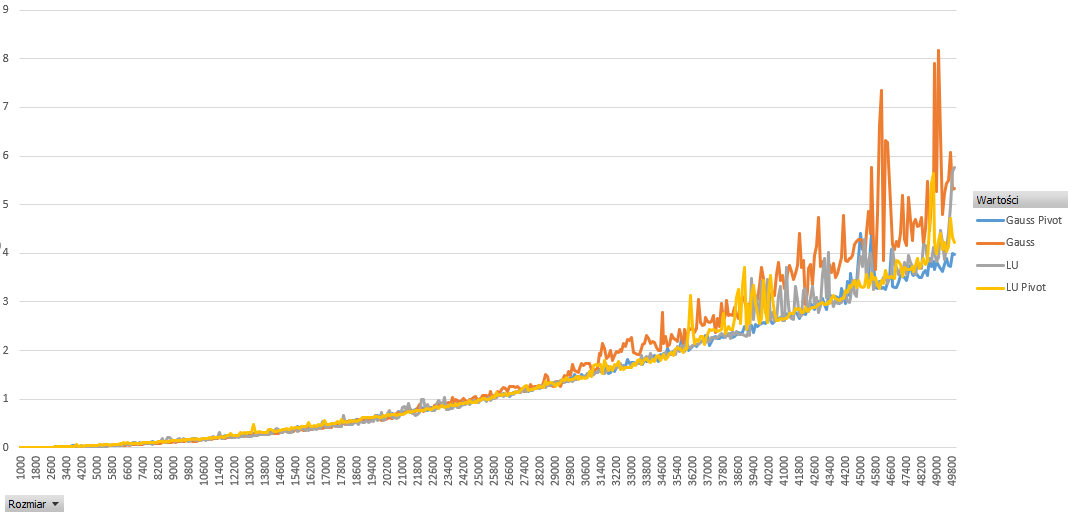
\includegraphics[scale=0.5]{wykres1}
      \centering
      \caption{Osiągniecia czasowe zaimplementowanych algorytmów}
  \end{figure}
  \textbf{UWAGA:} Otrzymane wyniki mogą być narażone na błąd spowodowany innymi procesami działającymi w tle w trakcie wykonywania testów! \\
  \begin{figure}[H]
    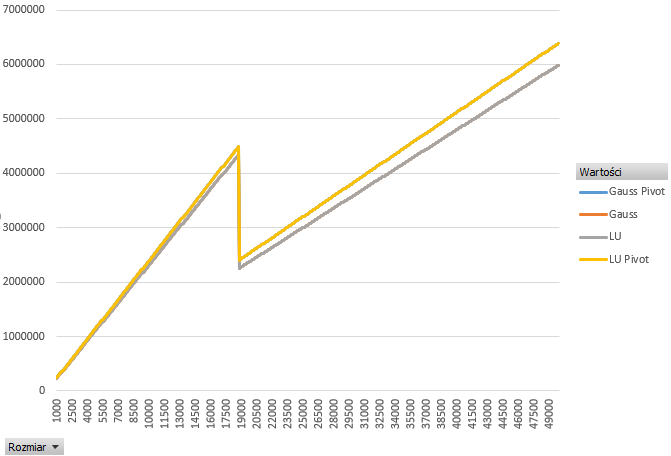
\includegraphics[scale=0.5]{wykres2}
      \centering
      \caption{Użyta pamięć w zaimplementowanych algorytmów}
  \end{figure}
  \begin{table}[H]
    \begin{tabular}{|c | c | c | c | c |} 
     \hline
     / &  $n=16$ & $n=10000$ & $n=50000$\\ [0.5ex] 
     \hline\hline
     Gauss & 1.3189010295585306e-15 & 5.166229763032209e-12 & 4.920922321731882e-14 \\
     Gauss Pivot & 2.8576114088871287e-16 & 4.443944163031559e-16 & 4.556461336521988e-16 \\ 
     LU & 1.3189010295585306e-15 & 5.166229763032209e-12 & 4.920922321731882e-14 \\ 
     LU Pivot & 2.8576114088871287e-16 & 4.443944163031559e-16 & 4.556461336521988e-16\\ 
     \hline
    \end{tabular}
    \caption{Wartości błędów względnych dla danych podanych wraz z treścią zadania}
    \end{table}
  \textbf{Interpretacja}: Patrząc na wykres odpowiadający za złożoność pamięciową zaimplementowanych algorytmów zauważamy, iż faktycznie ów złożoność jest liniowa, natomiast niepokój budzą wyniki odnośnie czasu. Zauważamy tendencję paraboliczną dla ów implementacji, co wskazuje na to, że w praktyce ta złożoność liniowa nie jest. Spowodowane jest to faktem, iż dyksretnie założyliśmy stałość wszystkich operacji wykonywanych wewnątrz pętel \textbf{FOR}, jednakże okazuje się, iż dostęp do elementów znajdujacych się w \textit{SparseArray} stały nie jest, co odciska swoje piętno na złożności czasowej całego algorytmu. W celu uzyskania złożoności liniowej należałoby skorzystać z innej struktury, lub utworzyć własną, która bierze pod uwagę specyfikację badanych macierzy.

\chapter{Wnioski}
  Porównując otrzymane wyniki zauważamy, iż sposób z wykorzystaniem częściowego wyboru elementu głównego zwraca poprawniejsze wyniki, z mniejszym błędem względnym, kosztem nieznacznie większego zużycia pamięci. Czasowo funkcje realizowane są w bardzo podobnym tempie. Dodatkowo zauważamy, iż algorytmy z częściowym wyborem radzą sobie w sytuacji, gdy na przekątnej znajdują się elementy zerowe, czego niestety nie można powiedzieć o ich odpowiednich bez wcześniejszych rotacji.
\end{document}